L'utilizzo del multi-cloud introduce una significativa complessità causata dalla mancanza di standardizzazione fra i vari Cloud Provider. Ogni Cloud Provider fornisce strumenti e metodi proprietari per accedere ai servizi, anch'essi differenti tra loro. Di conseguenza, anche se da una parte risulta molto vantaggioso l'utilizzo del multi-cloud, da un'altra parte risulta essere una tecnologia molto difficile da utilizzare. Questo porta alla ricerca di una soluzione che renda l'utilizzo del multi-cloud più semplice, in modo tale da astrarre e quindi rendere omogenea l'interazione con servizi offerti da diversi Cloud Provider, portando così lo sviluppatore a dover conoscere solo il servizio che viene utilizzato, ignorando le specifiche API necessarie per poterlo utilizzare. \\
In questo contesto nasce \textbf{FLY}, un \textbf{Domain-Specific Language} per il Calcolo Scientifico sul multi-cloud che ha l’obiettivo di semplificare lo sviluppo di applicazioni che sfruttino la potenza computazionale offerta da molteplici Cloud Provider. Il maggiore vantaggio di FLY è permettere a qualsiasi utente di sfruttare a pieno le potenzialità del multi-cloud astraendo l'interazione con il Provider, che viene totalmente gestita dal linguaggio \cite{isislab}. \\
L’aspetto più importante che racchiude il concetto di astrazione, è il concetto di \textbf{funzione FLY}, un blocco di codice indipendente eseguito in modo concorrente mediante i servizi FaaS. Le funzioni FLY vengono in un primo momento tradotte in linguaggio JavaScript o Python, in base ad una scelta dello sviluppatore, e successivamente deployate sul servizio serverless del Cloud Provider scelto dall'utente ed eseguite. Una volta terminata l'esecuzione del programma FLY, tutte le risorse allocate verrano eliminate, comprese quindi tutte le funzioni deployate durante l'esecuzione. \\
Le caratteristiche principali di FLY sono potenza, efficacia ed efficienza:
\begin{itemize}
    \item \textit{potente} - permette di sfruttare le capacità di computazione di diversi Cloud Provider in una singola applicazione. FLY gestisce in modo del tutto automatico l'allocazione e il rilascio delle risorse neccessarie;
    \item \textit{efficace} - risulta un linguaggio user-friendly con una sintassi molto simile ai linguaggi Java, Javascript, Python e R;    
    \item \textit{efficiente} - consente all'utente finale di concentrarsi solo sulla logica applicativa ignorando l'intera interazione con i diversi Cloud Provider.
\end{itemize}
In questo capitolo saranno descritti i dettagli del linguaggio FLY, in particolare gli obiettivi per cui è stato sviluppato e il suo funzionamento, introducendo inoltre il concetto di Domain-Specific Language (DSL) e Xtext, il framework utilizzato per lo sviluppo di FLY.

\section{Obiettivi}
FLY nasce con lo scopo di semplificare lo sviluppo di applicazioni Serverless di Calcolo Scientifico che sfruttino il sistema multi-cloud ottenendo un'alta scalabilità. \\
I principali obiettivi di FLY sono:
\begin{itemize}
    \item \textit{espressività} - essere espressivo all'interno del dominio del Calco Scientifico in modo da rendere lo sviluppo di un programma su larga scala semplice ed intuitivo anche per sviluppatori non esperti;
    \item \textit{alta usabilità} - permettere agli utenti esperti del dominio di riferimento di scrivere un programma FLY che sfrutti la potenza del multi-cloud in modo semplice ed intuitivo, grazie alla completa astrazione dell'interazione con i diversi Cloud Provider;    
    \item \textit{scalabilità} - permette di scalare facilmente sia su architetture Symmetric Multiprocessing (SMP) sia su architetture costruite su Cloud che supportano come modello di servizio FaaS, senza la necessità di conoscere le risorse che occorrono per l'esecuzione.
\end{itemize}

\section{Domain-Specific Language}
Un Domain-Specific Language (DSL) è un linguaggio di programmazione creato per un contesto specifico di applicazione. I DSL si differenziano dai più comuni linguaggi general-purpose che invece sono progettati per essere utilizzati per ogni dominio di applicazione. Per questo motivo, un linguaggio DSL, nasce con l'obiettivo di risolvere un problema specifico utilizzando una sintassi facile da imparare e semplice da utilizzare. I DSL più comuni in circolazione sono testuali, ma esistono anche DSL grafici. Tra i DSL più comuni troviamo l'HTML progettato per la costruzione di siti web, il CSS progettato per la creazione di stile di pagine HTML, l'SQL per la scrittura di query su database di tipo relazionali, e molti altri ancora. \\
I DSL permettono agli esperti di dominio di creare soluzioni software efficaci senza la necessità di avere competenze tecniche specifiche. 

\subsection{Xtext}
\textbf{Xtext} \cite{xtext} è un plugin open source per l'IDE Eclipse, nato per lo sviluppo di linguaggi di programmazione e DSL. Grazie a Xtext è possibile scrivere la grammatica del linguaggio e creare il parser, implementare regole di typing e scoping e generare un class model per l’Abstract Syntax Tree, fornendo anche un ambiente di sviluppo, basato su Eclipse completo di tutti gli aspetti classici dell'IDE. Il plugin è stato utilizzato per la creazione del compilatore di FLY per via degli innumerevoli vantaggi derivanti dal suo utilizzo.

\section{Architettura}
Un programma scritto in FLY viene tradotto in automatico dal compilatore in codice Java. Il programma Java orchestra tutto il funzionamento del programma FLY, dalla sua esecuzione all'allocazione di tutte le risorse necessarie al suo funzionamento. Nella \figurename~\ref{fig:esecuzione} viene mostrato il flusso di esecuzione di un programma FLY.
\begin{figure}[htbp]
 \centering
 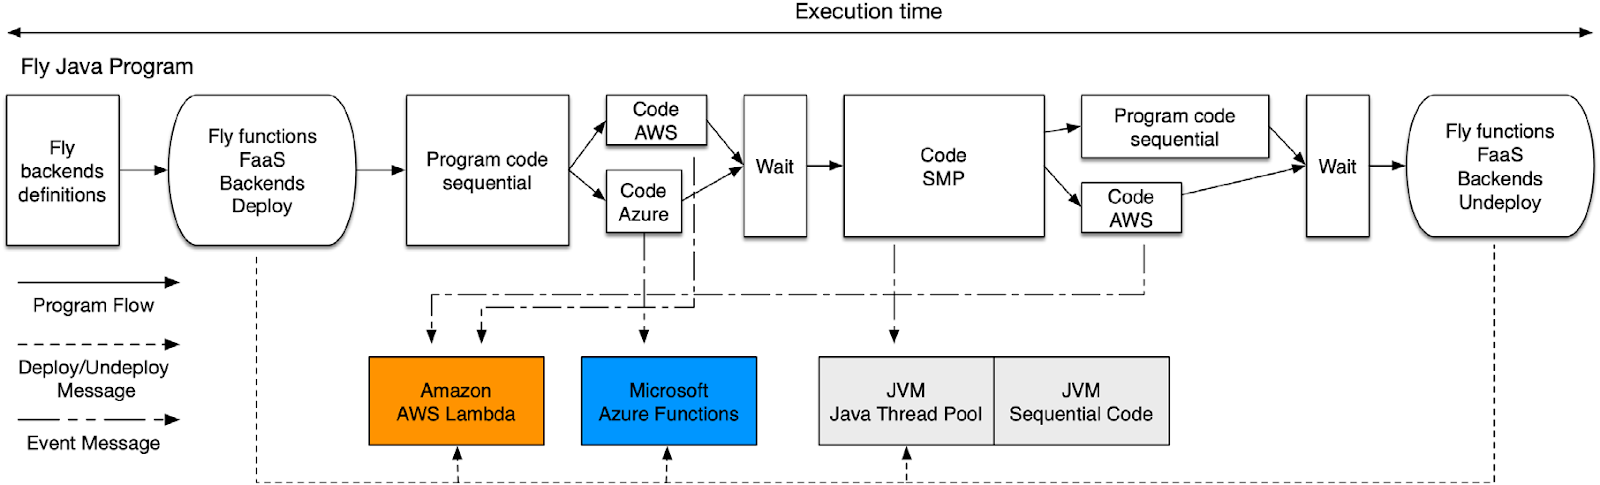
\includegraphics[scale=0.22]{./Figure/FLYEsecuzione.png}
 \caption{Flusso di esecuzione di FLY.}
 \label{fig:esecuzione}
\end{figure}
La prima fase prevede l'inizializzazione degli ambienti di esecuzione dichiarati all'interno del codice FLY, provvedendo ad effettuare il login sui diversi Cloud Provider utilizzati, tramite le credenziali di accesso specificate all'interno del codice FLY, e l'istanziazione dei servizi necessari. Nella seconda fase di esecuzione di un programma FLY, tutte le funzioni FLY dichiarate all'interno del codice vengono tradotte in linguaggio JavaScript o Python, in base ad una scelta effettuata dallo sviluppatore previa esecuzione, e successivamente caricate sul rispettivo ambiente Cloud. Una volta terminate queste due fasi di inizializzazione, il programma principale viene mandato in esecuzione. Al suo termine vengono eseguite le operazioni necessarie per eliminare tutte le istanze dei servizi Cloud allocati in precedenza.

\section{Definizione del linguaggio}
FLY mette a disposizione dell'utente una serie di costrutti specifici che lo aiutano nella costruzione di applicazioni di calcolo scientifico su multi-cloud. Esse comprendono sia tipi di dati specifici per specificare risorse o l'ambiente di esecuzione, ma anche metodi di comunicazione e esecuzione specifici. \\
Il Listato~\ref{lst:pigreco} mostra un esempio di programma FLY per il calcolo di una stima del PI Greco utilizzando il metodo Monte Carlo, sfruttando il servizio AWS Lambda  \cite{lambdasite}. Quest'ultimo verrà utilizzato come supporto all'introduzione dei vari elementi che compongono il linguaggio FLY nei capitoli successivi.
\begin{lstlisting}[language=FLY,caption={Stima di PI Greco usando il metodo Monte Carlo su ambiente AWS.}, label={lst:pigreco}]
var Local = [type="smp", nthread=4]

var Cloud = [type="aws", profile="user_name", access_id_key = "access_id_key", secret_access_key="secret_access_key", region="eu-west-2", language="nodejs12.x", nthread=2, memory=256, seconds=300]

var ch = [type="channel"] on Cloud

func hit(){	
    var r = [type="random"]
    var x = r.nextDouble()
    var y = r.nextDouble()
    var msg = 0
    
    if((x * x) + (y * y) < 1.0) { msg = 1 }
    ch!msg on Cloud
}


func estimation(){
    var sum = 0
    var crt = 0
    for i in [0:100] {
        sum += ch? as Integer
        crt += 1
    }
    println "pi estimation: " + (sum * 4.0) \ crt
}

fly hit in [0:100] on Cloud thenall estimation  
\end{lstlisting}  

\subsection{Tipi di dati}
In FLY è possibile raggruppare i diversi tipi di dati in due insiemi: \textbf{basici} e \textbf{di dominio}. \\
Il primo insieme comprende i tipi di dati:
\begin{itemize} 
    \item \textit{interi} - numeri interi appartenenti all’intervallo [-2147483648, 2147483647];
    \item \textit{reali} - numeri in virgola mobile in doppia precisione secondo la specifica IEEE 754 \cite{ieee};
    \item \textit{stringhe} - sequenze di caratteri unicode (UTF-16) \cite{utf};
    \item \textit{booleani} - un valore tra \verb|true| o \verb|false|.
\end{itemize}
Con questi tipi di dati è possibile inizializzare una variabile oppure dichiarare array monodimensionali, bidimensionali e tridimensionali composti da elementi omogenei al tipo usato per la dichiarazione. Nel listato~\ref{lst:pigreco} le variabili \verb|msg|, \verb|sum| e \verb|crt| utilizzano dati di tipo basico, ovvero interi. \\
Il secondo insieme comprende un gruppo di dati che permettono all'utente di interagire e comunicare con l'ambiente di esecuzione. Le variabili \verb|local|, \verb|cloud|, \verb|ch| e \verb|r| sono variabili di tipo dominio. Le variabili \verb|local| e \verb|cloud| vengono utilizzate per dichiarare un'\textbf{ambiente di esecuzione}, necessario per permettere a FLY di configurare le risorse utili al funzionamento dell'applicazione. La variabile \verb|ch| viene utilizzata per dichiarare un \verb|channel|, oggetto necessario per la comunicazione e la sincronizzazione tra le varie funzioni FLY. Queste due tipologie di variabili di dominio verranno descritte nei capitoli a seguire. La variaibile \verb|r| è un istanza di un oggetto di tipo \verb|random|. Di seguito sono riportare le righe di codice relative all'utilizzo della variabile \verb|r| all'interno del Listato~\ref{lst:pigreco}.
\begin{lstlisting}[language=FLY,firstnumber=9,label={lst:r},belowskip=-0.8 \baselineskip]
    var r = [type="random"]
    var x = r.nextDouble()
    var y = r.nextDouble()
\end{lstlisting}
Al rigo 9 viene istanziato l'oggetto di tipo \verb|random|. La dichiarazione di una variabile di dominio necessita di una serie di parametri che variano in base al tipo di oggetto che si intende istanziare, eccetto per il primo parametro, ovvero \verb|type|, che ne identifica il tipo. Nelle due righe successive l'oggetto \verb|r| viene utilizzato per generare due reali casuali, tramite l'utilizzo del metodo \verb|nextDouble()|. In questo modo otteniamo due reali casuali compresi fra 0 e 1, memorizzati rispettivamente nelle variabili \verb|x| e \verb|y|. All'interno dell'algoritmo queste due variaibili identificano le coordinate del punto generato casualmente all'interno del quadrato.

\subsection{Ambiente di esecuzione}
Per permettere il corretto funzionamento di un programma FLY è neccesario dichiarare gli \textbf{ambienti di esecuzione}. Per ogni programma FLY è richiesta la dichiarazione di un ambiente di esecuzione locale, corrispondente alla macchina su cui viene eseguito il programma, in modo da permette a FLY la parallelizzazione del programma sfruttando al meglio il numero di thread di cui la macchina dispone. Oltre alla dichiarazione di un ambiente di esecuzione locale, è possibile dichiararne altre tre tipologie:
\begin{itemize}
    \item \textit{aws} - ambiente su Cloud legato al provider Amzon Web Services (AWS) che sfrutta il servizio AWS Lambda \cite{lambdasite} per eseguire le funzioni FLY;
    \item \textit{aws-debug} - simulazione in locale dell'ambiente di esecuzione di AWS;
    \item \textit{azure} - ambiente su Cloud legato al provider Microsoft Azure \cite{MicrosoftSite} che sfrutta il servizio Azure Function \cite{FunctionSite} per eseguire le funzioni FLY.
\end{itemize}
Gli ambienti di esecuzione permettono allo sviluppatore di scegliere su quale ambiente eseguire le funzioni FLY. È importante ricordare che le funzioni FLY per essere eseguite su ambienti Cloud devono essere tradotte in un linguaggio supportato dal Cloud Provider, per questo motivo è richiesto all'utente di specificare il linguaggio di programmazione in cui esse verranno tradotte. Nel Listato~\ref{lst:pigreco} le prime 3 righe del codice, riportate di seguito, contengono la dichiarazione dei due ambienti di esecuzione utilizzati: ambiente locale e ambiente AWS.
\begin{lstlisting}[language=FLY,label={lst:r},belowskip=-0.8 \baselineskip]
var Local = [type="smp", nthread=4]

var Cloud = [type="aws", profile="user_name", access_id_key = "access_id_key", secret_access_key="secret_access_key", region="eu-west-2", language="nodejs12.x", nthread=2, memory=256, seconds=300]
\end{lstlisting}

\subsection{Channel}
I channel sono lo strumento necessario per permettere la comunicazione tra le varie funzioni FLY. La dichiarazione di un oggetto di tipo \verb|channel| necessita la specifica dell'ambiente di esecuzione sul quale funzionare mediante la parola chiave \verb|on|. Questo metodo di comunicazione segue il modello delle code di messaggi bloccanti: il processo mittente attende la trasmissione del messaggio sulla rete. La comunicazione tramite canale in FLY avviene con l'utilizzo di due caratteri: \verb|"!"| e \verb|"?"|. Il carattere \verb|"!"| permette l'invio di messaggi sul canale, il carattere \verb|"?"| permette, invece, di prelavare un messaggio dalla coda. Di seguito sono riportati gli utilizzi del carattere \verb|"!"| e \verb|"?"| all'interno del Listato~\ref{lst:pigreco}.
\begin{lstlisting}[language=FLY,firstnumber=7,label={lst:r},belowskip=-0.8 \baselineskip]
func hit(){	
    var r = [type="random"]
    var x = r.nextDouble()
    var y = r.nextDouble()
    var msg = 0
    
    if((x * x) + (y * y) < 1.0) { msg = 1 }
    ch!msg on Cloud
}
\end{lstlisting}
\begin{lstlisting}[language=FLY,firstnumber=18,label={lst:r},belowskip=-0.8 \baselineskip]
func estimation(){
    var sum = 0
    var crt = 0
    for i in [0:100] {
        sum += ch? as Integer
        crt += 1
    }
    println "pi estimation: " + (sum * 4.0) \ crt
}
\end{lstlisting}

\subsection{Esecuzione funzioni FLY}
Per poter eseguire una funzione FLY è necessario utilizzare la parola chiave \verb|fly| in modo da specificare la funzione che si intende eseguire, il numero di volte che questa funzione deve essere eseguita e l'ambiente di esecuzione sul quale verrà eseguita. Inoltre, è possibile utilizzare la parola chiave \verb|then| o \verb|thenall| in modo da specificare una funzione di Callback. Le funzioni di Callback sono funzioni FLY che vengono eseguite in locale al termine dell'esecuzione di una precedente funzione. Utilizzando la parola chiave \verb|then| la funzione di Callback verrà eseguita al termine di ogni singola funzione FLY, mentre, utilizzando la parola chiave \verb|thenall|, la funzione di Callback verrà eseguita solo al termine di tutte le funzioni FLY. Di seguito è riportato l'utilizzo della parola chiave \verb|fly| all'interno del nostro esempio.
\begin{lstlisting}[language=FLY,firstnumber=28,label={lst:r},belowskip=-0.8 \baselineskip]
fly hit in [0:100] on cloud thenall estimation  
\end{lstlisting}
Analizziamo ora la sintassi utilizzata:
\begin{itemize}
    \item la parola chiave \verb|fly| seguita dal nome della funzione \verb|hit| indica quale funzione si intende eseguire;
    \item la parola chiave \verb|in| seguita dall'intervallo \verb|[0:100]| indica, in questo caso, che la funzione \verb|hit| deve essere eseguita 100 volte. In generale l'intervallo \verb|[0:n]| indica che la funzione deve essere eseguita \textit{n}  volte;
    \item la parola chiave \verb|on| seguita dalla variabile \verb|cloud|, sta a indicare che la funzione \verb|hit| verrà eseguita sull'ambiente di esecuzione rappresentato dalla variabile \verb|cloud|, ovvero AWS;
    \item la parola chiave \verb|thenall| seguita dal nome della funzione \verb|estimation| indica che, al termine delle 100 esecuzioni della funzione \verb|hit|, verrà eseguita la funzione \verb|estimation|. 
\end{itemize}

\subsection{Struttura di un progetto FLY}
FLY utilizza il gestore di progetti Java \textbf{Maven} \cite{maven} per la costruzione dei progetti FLY. Maven è uno strumento basato sulla presenza del file pom.xml, acronimo di \textbf{Project Object Model}, che ha il compito di definire identità, struttura del progetto e dipendenze necessarie al funzionamento dell'applicazione. \\
La creazione di un progetto FLY comporta la generazione di un progetto Java Maven che include:
\begin{itemize}
    \item la cartella \textit{src} in cui è situato il file con estensione \textit{.fly} contenente il codice del programma scritto in linguaggio FLY;
    \item la cartella \textit{src-gen} destinata a contenere i file generati dal compilatore;
    \item il file \textit{pom.xml} per la gestione del progetto e specifica delle librerie necessarie per l'esecuzione del programma.
\end{itemize}
